\newpage
\section{2024年10月30日}
\begin{tcolorbox}[cyan]
    \begin{description}
        \item[\large \textbf{任务}]
        \item[1、] 将GCOPTER-MINCOS代码移植至EGO-PLANNER-V2
        \item[2、] 继续复现Polynomial-based 其余部分(动态环、拓扑路径规划)
    \end{description}
\end{tcolorbox}
\subsection{将GCOPTER-MINCOS代码移植至EGO-PLANNER-V2}
(1)\textbf{设计状态机FSM}


在原有状态机的基础上增加
\textbf{环的距离检测}和\textbf{固定航点重规划}。

具体逻辑:在检测到到达环(航点)附近时,规划到下一个航点的全局轨迹;
获得下一段全局轨迹之后,获得该段轨迹的局部路径规划目标点,最后进行固定航点重规划。
在飞行至环中心时,切换至原有重规划。
\begin{algorithm}[htbp]  
    \caption{\ 固定航点重规划}  
    \label{fsm}  
    \begin{algorithmic}[1]   
      \Require  无人机位置$odom\_pos\_$, 圆环中心位置$circle\_pos\_$, 固定航点重规划标志$touch\_circle\_$,当前时间$time\_now\_$,重规划界限$planning\_horizen\_$,全局规划界限$no\_replan\_thresh\_$,当前目标点$goal$
    %   \Ensure  
    \State \CASE{$ EXEC\_TRAJ $}
    \If{ $touch\_circle\_  \ \ \mathbf{and}\ \  (time\_now\_ > circle\_cross\_time\_ - 0.1\ \  \mathbf{or}\ \  (odom\_pos\_ - circle\_pos\_).norm() < 0.09)$}
            \State $cir\_ps\_.erase(cir\_ps\_.begin())$
            \State $touch\_circle\_ = false$
            \State $already\_cross = true$
            \State $have\_planed\_next\_waypoint = false$
        \EndIf
        \If{ $(goal - odom\_pos\_).norm() < no\_replan\_thresh\_\ \ \mathbf{and}\ \ planNextWaypoint()$}
            \State $have\_planed\_next\_waypoint = true$
            \If{ $!cir\_ps\_.empty()\ \ \mathbf{and}\ \ (odom\_pos\_ - circle\_pos\_).norm() < planning\_horizen\_$}
            \State $touch\_circle\_ = true$
            \State $planFromLocalTraj(1)$
            \EndIf
        \EndIf
    \end{algorithmic}  
  \end{algorithm}


(2)\textbf{定义MINCOS类}


(3)\textbf{增加固定航点重规划算法}


(4)\textbf{运行效果}


正常运行效果,如图\ref{image2}。
\begin{figure}[htbp]
    \centering
    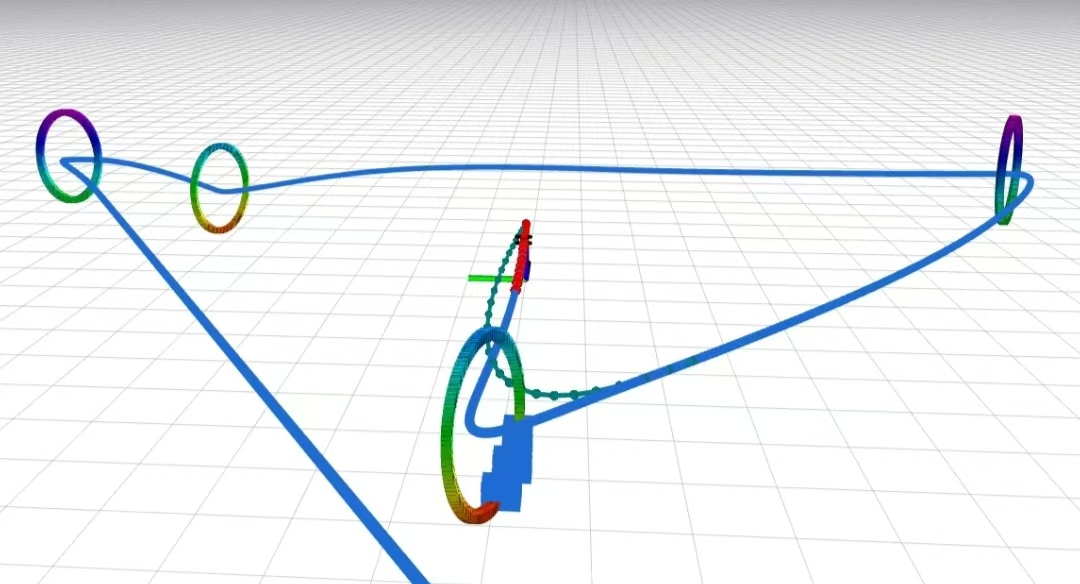
\includegraphics[width=16cm, height=7cm]{image/2.jpg}
    \caption{航点硬约束的局部路径规划全局效果图}\label{image2}
\end{figure}\\


有小概率优化之后的轨迹会打圈,并且很难从环的另一端钻出,如图\ref{image3},初步分析可能原因:


一方面是逻辑还需修改,因为固定经过环的中心即可,在需要大幅转弯时,可能存在掉头飞行的情况。


另一方面可能是优化的代价函数需修改,所采用的优化代价函数的每一项代价是采用EGO-V2的代价函数进行计算的,可能并不适用于固定航点优化。


\begin{figure}[htbp]
    \centering
    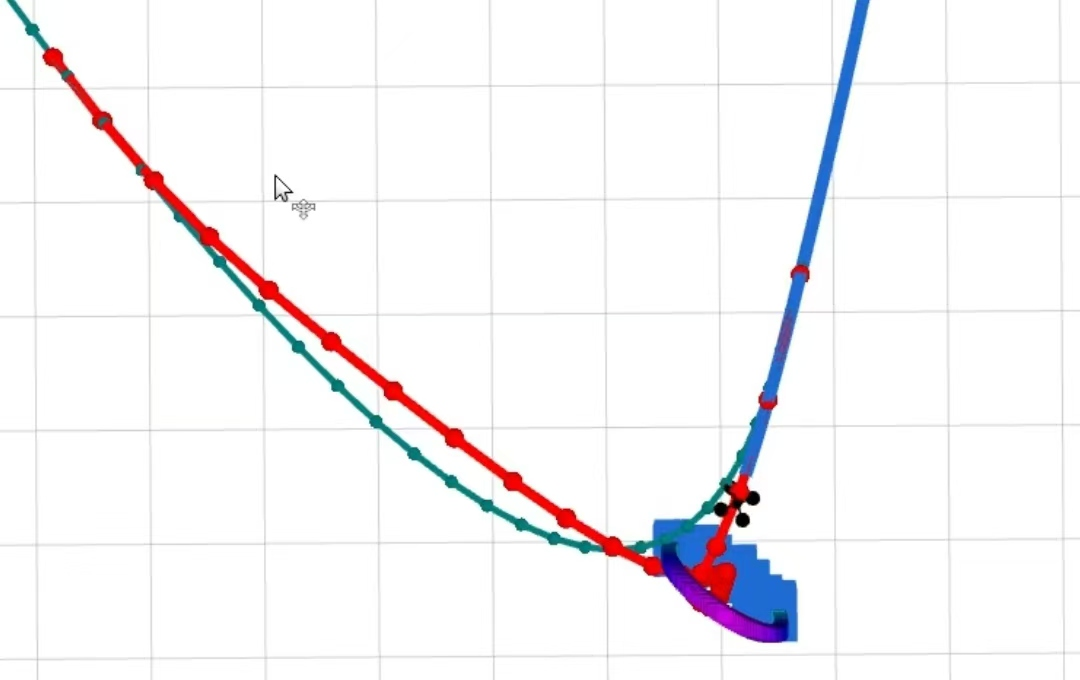
\includegraphics[width=14cm, height=8cm]{image/3.jpg}
    \caption{航点硬约束的局部路径规划失败图}\label{image3}
\end{figure}
\subsection{Time-Optimal Gate-Traversing Planner for Autonomous Drone Racing(ICRA2024)}
Code: https://github.com/FSC-Lab/TOGT-Planner
\subsubsection{论文所解决的问题}
根据所提供的门的信息,不考虑环境中的其他环境信息,计算出一条穿过所有门的时间最优且符合无人机动力学的全局轨迹。
\subsubsection{论文算法}
(1)\textbf{四旋翼无人机模型}


状态变量:$\mathbf{x} = [\mathbf{p}^W,\mathbf{q}_{WB},\mathbf{v}^W,\boldsymbol{\omega}^B]^T\in\mathbb{R}^n,n=13$,分别为世界坐标系下的位置、由机体坐标系到世界坐标系的单位四元数旋转矩阵、世界坐标系下的速度、机体坐标系下的角速度\\


输入变量:$\mathbf{u}=[f_1,f_2,f_3,f_4]^T\in \mathbb{R}^m,m=4$,依次为四个电机的推力
\begin{align}
    \dot{\mathbf{p}}  =\mathbf{v},&\quad\dot{\mathbf{q}}=\frac12\boldsymbol{\Lambda}(\mathbf{q})\left[\begin{array}{c}0\\ \boldsymbol{\omega}\end{array}\right],\\ 
    \dot{\mathbf{v}}  =\mathbf{g}+\frac1m\mathbf{R}(\mathbf{q})\mathbf{F}_{T},&\quad\dot{\boldsymbol{\omega}}=\mathbf{J}^{-1}(\boldsymbol{\tau}-\boldsymbol{\omega}\times\mathbf{J}\boldsymbol{\omega})
\end{align}
其中 
\begin{equation}
    \mathbf{F}_{T}  =\left[\begin{array}{c}0\\ 0\\ \sum f_{i}\end{array}\right],\boldsymbol{\tau}=\left[\begin{array}{c}l(f_1+f_2-f_3-f_4)\\ l(-f_1+f_2+f_3-f_4)\\ c_{\tau}(f_1-f_2+f_3-f_4)\end{array}\right].
\end{equation}
(2)\textbf{门约束的定义}\\
\textbf{球形门}:指在飞行过程中必须要经过的航点。
\begin{equation}
    \mathcal{G}_{\mathcal{B}}=\{\mathbf{p}\in\mathbb{R}^3|\|\mathbf{p}-\mathbf{p}_w\|_2\leq\delta\},
\end{equation}
其中,$\mathbf{p}_w$是球形门的中心,$\delta$是其半径。\\
\textbf{凸多边形门}:指在飞行过程中要钻过的门或隧道。
\begin{equation}
    \mathcal{G}_{\mathcal{P}}=\{\mathbf{p}\in\mathbb{R}^3|\mathbf{A}\mathbf{p}\leq\mathbf{b}\},
\end{equation}
(3)\textbf{时间最优门遍历问题}
\begin{align}
\min_{\mathbf{x},\mathbf{u},t_f}& t_{f} \\
\mathrm{s.t.}& \mathbf{x}(0)=\bar{\mathbf{x}}_0, \mathbf{x}(t_f)=\bar{\mathbf{x}}_f, \\
&\dot{\mathbf{x}}=\mathbf{f}(\mathbf{x},\mathbf{u}), \mathbf{h}(\mathbf{x},\mathbf{u})\leq0, \\
&\exists 0<t_{1}<t_{2}<...<t_{L}<t_{f}, \\
&\mathbf{h}_{\mathcal{G}^{i}}(\mathbf{p}_{\mathbf{x}(t_{i})})\leq0, 1\leq i\leq L,
\end{align}
(4)\textbf{问题转化与求解}\\
\textbf{门约束与时间解耦}
\begin{equation}
    \begin{aligned}\min_{\mathbf{P},\mathbf{T}}&T_{\Sigma}+I_{\mathcal{T}(\mathbf{P})}(\mathbf{T})\\\mathrm{s.t.}&\mathbf{h}_{\mathcal{G}^{i}}(\mathbf{p}_{i})\leq\mathbf{0}, 1\leq i\leq L,\end{aligned}
\end{equation}
其中,
\begin{equation}
    I_{\mathcal{T}(\mathbf{P})}(\mathbf{T})=\left\{\begin{array}{ll}0&,\mathrm{if~}\mathbf{T}\in\mathcal{T}(\mathbf{P})\\
        \infty&,\mathrm{if~}\mathbf{T}\notin\mathcal{T}(\mathbf{P})\end{array}\right.
\end{equation}
\begin{equation}
    \begin{aligned}\label{TP}
\mathcal{T}(\mathbf{P})=\{\mathbf{T}\in\mathbb{R}_{>}^{L+1}& \mid\exists\mathbf{x},\mathbf{u}:[0,T_\Sigma]\to\mathbb{R}^n,\mathbb{R}^m \\
\text{s.t.}& \mathbf{x}(0)=\bar{\mathbf{x}}_{0}, \mathbf{x}(T_{\Sigma})=\bar{\mathbf{x}}_{f} \\
&\dot{\mathbf{x}}=\mathbf{f}(\mathbf{x},\mathbf{u}),\mathbf{h}(\mathbf{x},\mathbf{u})\leq0 \\
&\mathbf{p}_{\mathbf{x}(t_{\Sigma_{i}})}=\mathbf{p}_{i}, 1\leq i\leq L\}.
\end{aligned}
\end{equation}
给定门的位置向量后,可行时间分配向量的集合如式\ref{TP}所示。采用MINCO轨迹能够消除尽可能多的约束,并且具有最少数量的系数,大大降低了问题的复杂性。
通过结合微分平坦特性消除对系统动力学、初始状态和终端状态的约束,而且可以确保精确的航路点遍历,从\ref{TP}中删除大量约束,只留下状态输入约束。
连续状态输入约束通过采样来定义惩罚泛函。
\begin{equation}
    \begin{aligned}
&I_{\hat{\mathcal{T}}(\mathbf{P})}(\mathbf{T})=\int_{0}^{T_{\Sigma}}\mathrm{max}[\mathbf{h}_{\Psi}(\mathbf{y}^{[s]}(t)),\mathbf{0}]^{3}dt, \\
&\approx\sum_{i=1}^{L+1}\sum_{j=0}^{\kappa_i}\max[\mathbf{h}_\Psi(\mathbf{y}^{[s]}(t_{i-1}+j\Delta t_i)),\mathbf{0}]^3\Delta t_i,
\end{aligned}
\end{equation}
(5)\textbf{门约束和时间约束}


通过将门约束和时间约束的可行解空间映射至n维欧式空间后,进行无约束优化。\\
(6)\textbf{无约束优化}
\begin{equation}
    \min_{\mathbf{D},\mathbf{K}}\quad T_{\Sigma}(\mathbf{K})+I_{\hat{\mathcal{T}}(\mathbf{P}(\mathbf{D}))}(\mathbf{T}(\mathbf{K})).
\end{equation}
推导上述函数梯度,并采用L-BFGS算法进行优化,优化完成后可由$\mathbf{D、K}$获得航点向量$\mathbf{P}$和时间向量$\mathbf{T}$,然后构建MINCO轨迹,之后通过微分平坦便可得到全状态变量和输入变量。
\subsubsection{论文启发}
本篇论文通过对穿过所有门的全局路径规划问题进行问题建模,并且采用MINCO轨迹来进行轨迹表示,
一方面能够减少优化问题中的约束,另一方面可以减少优化参数;对连续性状态输入约束采用离散化的惩罚泛函;对凸的门约束和时间约束映射至n维欧氏空间进行优化。
从本篇论文中能够了解MINCO轨迹以及几何优化方法的应用。
